% ------------------------------------------------------------------------
% == Modelo de Relatório Técnico/Acadêmico em conformidade com 
% == ABNT NBR 10719:2015 Informação e documentação -
% == Relatório técnico e/ou científico
% ------------------------------------------------------------------------
% == Adapatado para modelo do CPAI
% ------------------------------------------------------------------------

\documentclass[
	12pt,				  % tamanho da fonte
	%openright,	  % capítulos começam em pág ímpar (insere página vazia caso preciso)
	%twoside,			% para impressão em recto e verso. Oposto a oneside
  oneside,			% para impressão em recto e verso. Oposto a twoside
	a4paper,			% tamanho do papel. 
	english,			% idioma adicional para hifenização
	french,				% idioma adicional para hifenização
	spanish,			% idioma adicional para hifenização
	brazil,				% o último idioma é o principal do documento
	]{abntex2}

% ---
% Pacotes em pasta própria para deixar o documento mestre limpo
\usepackage{sty/pacotes}

% ---
% Informações de dados sobre o Relatório
% == IMPORTANTE ABRIR E ALTERAR OS DADOS DESTE ARQUIVO!
\usepackage{sty/info}

% Início do documento
\begin{document}
  % Seleciona o idioma do documento (conforme pacotes do babel)
  %\selectlanguage{english}
  \selectlanguage{brazil}
  
  % Retira espaço extra obsoleto entre as frases.
  \frenchspacing 
  
  % ----------------------------------------------------------
  % == ELEMENTOS PRÉ-TEXTUAIS
  % ----------------------------------------------------------
  % \pretextual
  
  % ---
  % Capa
  \imprimircapa

  % ---
  % Folha de rosto (o * indica que haverá a ficha bibliográfica)
  \imprimirfolhaderosto*
  
  % ---
  % Anverso da folha de rosto
%  \include{pretextuais/creditos}
 
  
  % ---
  % Agradecimentos

  
  % ---
  % Resumo
   %----------------------------------------------------------------------------------------------------------------
% File : resumo.tex
%----------------------------------------------------------------------------------------------------------------

% resumo na língua vernácula (obrigatório)
\setlength{\absparsep}{18pt} % ajusta o espaçamento dos parágrafos do resumo
\begin{resumo}  
    
    Este estudo tem como base uma amostra de 500 alunos do 9º ano de 2017 do Brasil disponibilizada em um banco de dados da Prova Brasil realizada pelo Saeb em 2017. Com o objetivo de avaliar o ensino básico, através das notas dos alunos, realiza-se testes estatísticos para as relações das notas em Matemática com a regiões das escolas e das notas em Língua portuguesa com os tempos de uso de ''telas'' (Ex.: Televisores, celulares e entre outros), no qual com critérios de confiabilidade, obteve resultados de desigualdades regionais e pontuações nas notas influenciadas por fatores relacionados ao tempo de uso de telas.

    
  \noindent
  \textbf{Palavras-chaves}: \kwords
\end{resumo}

  
  % ---
  % inserir listas de ilustrações, tabelas e quadros
  %----------------------------------------------------------------------------------------------------------------
% File : itq.tex
%----------------------------------------------------------------------------------------------------------------

% ---
% inserir lista de ilustrações
\pdfbookmark[0]{\listfigurename}{lof}
\listoffigures*
\cleardoublepage

% ---
% inserir lista de tabelas
\pdfbookmark[0]{\listtablename}{lot}
\listoftables*
\cleardoublepage

  
  % ---
  % inserir listas de siglas
  %----------------------------------------------------------------------------------------------------------------
% File : siglas.tex
%----------------------------------------------------------------------------------------------------------------

% ---
% inserir lista de abreviaturas e siglas
\begin{siglas}
    \item[INEP]     Instituto Nacional de Estudos e Pesquisas Educacionais Anísio Teixeira
    \item[SAEB]     Sistema de Avaliação da Educação Básica
  \end{siglas}
  
  % ---
  % inserir lista de símbolos
  \begin{simbolos}
    \item[$ \sigma $]     Letra grega minúscula sigma
    \item[$ \mu $]        Letra grega minúscula mu
  \end{simbolos}
  
 
  
  % ---
  % inserir o sumario
  \pdfbookmark[0]{\contentsname}{toc}
  \tableofcontents*
  \cleardoublepage
  % ---

  % ----------------------------------------------------------
  % == ELEMENTOS TEXTUAIS
  \textual
  
  % ----------------------------------------------------------
  % Introdução
  %----------------------------------------------------------------------------------------------------------------
% File : introducao.tex
%----------------------------------------------------------------------------------------------------------------

% Introdução (exemplo de capítulo sem numeração, mas presente no Sumário)
\chapter*[Introdução]{Introdução}
\addcontentsline{toc}{chapter}{Introdução}

% Avaliação
Este documento tem como objetivo analisar os fatores sociais de alunos brasileiros do 9º ano de 2017,
sobre os quais avalia possibilidades de diferenças no desempenho do aprendizado básico destes.
Para a análise, serão utilizados dados do Sistema de Avaliação da Educação Básica (SAEB) de 2017 
divulgado pelo \citeonline{Saeb2017a)}. O banco de dados utilizado no estudo é constituído por dados de
estudantes do 9\textsuperscript{o} ano que realizaram a Prova Brasil no ano de 2017.

% Saeb
O SAEB avalia o desempenho em Matemática e Língua Portuguesa por meio de testes e questionários sobre fatores sociais de
alunos, aplicados bienalmente em redes públicas
e amostras de escolas privadas sobre turmas do 5º e 9º anos do ensino fundamental e 
3º ano do ensino médio.

% Amostra
Esta análise parte de uma amostragem aleatória simples de 5.271 alunos deste banco de dados, e relaciona 
fatores como raça/cor, sexo dos alunos, localizações das escolas e escolaridade da mãe destes, com as variáveis
a serem explicadas como a soma destas notas e o tempo de afazeres domésticos realizados por dia com base nos alunos.

% Banco de dados

A aplicação dos testes de hipóteses para a análise da amostra, bem como dos gráficos (para a análise descritiva), utiliza ferramentas
do software \textsc{R} nas versões 3.6.3 e 4.0.3. Parte do processamento dos dados foi feito com o software \textsc{Python} versão 3.7.3.\footnote{Pacotes externos usados para a manipulação dos dados:\\\textit{R: tidyverse, data.table, reshape2, patchwork, EnvStats, PMCMR; \\Python: pandas}}


  
  % ----------------------------------------------------------
  % == PARTE - preparação da pesquisa
  % ----------------------------------------------------------
  \part{FUNDAMENTAÇÃO}
  
  % ----------------------------------------------------------
  % Capitulo com exemplos de comandos inseridos de arquivo externo 
  %----------------------------------------------------------------------------------------------------------------
% File : exemplo.tex
%----------------------------------------------------------------------------------------------------------------

% ---
% Este capítulo, utilizado por diferentes exemplos do abnTeX2, ilustra o uso de
% comandos do abnTeX2 e de LaTeX.

\chapter{Metodologia}
% Relacao com notas
Como variáveis explicativas para a soma das notas, o estudo relaciona a raça/cor, a escolaridade da mãe e as localizações das escolas,
e avalia o quanto essas variáveis influenciam no desempenho na Prova Brasil. Para avaliar estas relações, um estudo prévio foi realizado
com amostras de tamanhos 30, 50 e 100 dos 5.271 alunos em que, com os testes \citeonline{anderson1954test}, \citeonline{shapiro1965analysis}
e \citeonline{shapiro1972approximate}, se concluiu que as distribuições das notas são normais. Este resultado será utilizado para atender
os testes paramétricos que pressupõem normalidade dos dados. Os testes a serem aplicados serão o teste ANOVA dado por \citeonline{fisher1928general} para 
avaliar os fatores com mais de 2 categorias e o teste t-Student para as comparações dois a dois \cite{o1908student}.
Estes testes utilizam das médias ($\mu$) de cada grupo para avaliar as distâncias significativas entre eles, no qual previamente avalia se as
variâncias ($\sigma^2$) destes são iguais (Teste B), através do teste proposto por \citeonline{bartlett1954note}.

% Relacao com afazeres
Quanto ao tempo gasto com afazeres domésticos, as variáveis a serem relacionadas são a raça/cor, a escolaridade da mãe
e o sexo, para observar se há indícios de diferenças sociais entre a disponibilidade de tempo em casa para outras possíveis 
tarefas na formação do aprendizado básico. Para estas relações, os testes estatísticos não paramétricos são apropriados,
e utiliza-se o teste de \citeonline{kruskal1952use} para fatores com mais de duas categorias (Teste K), e o
teste de \citeonline{mann1947test} para a comparação dois a dois das categorias (Teste W). Estes testes avaliam as
distribuições das informações com base na posição, para verificar se as distâncias entre as categorias são significativas.

% Avaliacao dos testes
Para avaliar os resultados dos testes, foi proposto o uso da correção de \citeonline{bonferroni1936teoria} para os 
testes com mais de duas categorias. Se houver evidências para rejeitar igualdade destas, a comparação dois a dois é
efetuada e a correção é utilizada. Esta correção é sobre o p-valor, que é avaliado em uma escala de significância,
adotado por este estudo como uma confiança de 95\%, no que diz respeito a aceitar a hipótese nula $H_0$.
  
  % ----------------------------------------------------------
  % == PARTE - Resultados
  % ----------------------------------------------------------
  \part{Resultados}
  
  % ---
  % Capitulo de revisão de literatura
  % File : rev_literatura.tex


\chapter{Comparações}
%%%%%%%%%%%%%%%%%%%%%%%%%%%%%%%%%%%%%%%%%%%%%%%%%%%%%%%%%%%%%%%%%%%%%%%%%%%%%%%%%%%%%%%%%%%%%%%%%%%%%%%%%%%
%%%%%%%%%%%%%%%%%%%%%%%%%%%%%%%%%%%% AFAZERES_DOM %%%%%%%%%%%%%%%%%%%%%%%%%%%%%%%%%%%%%%%%%%%%%%%%%%%%%%%%%
%%%%%%%%%%%%%%%%%%%%%%%%%%%%%%%%%%%%%%%%%%%%%%%%%%%%%%%%%%%%%%%%%%%%%%%%%%%%%%%%%%%%%%%%%%%%%%%%%%%%%%%%%%%
\section{Tempo em afazeres domésticos}
O tempo gasto com afazeres domésticos pode privar o aluno de exercer o estudo
do ensino básico. Foram feitas análises sociais com base nas diferenças entre os 
períodos de tempo gastos diariamente nestas atividades.

%%%%% Gráfico de Sexo por afazeres_domesticos
\begin{figure}[h]
    \label{sexo_afazeres}
    \caption{Proporção dos sexos por período de tempo em afazeres domésticos por parte
    dos alunos.\label{sexo_afazeres}} % Pra fazer ref, tem q estar no caption
    \begin{center}
        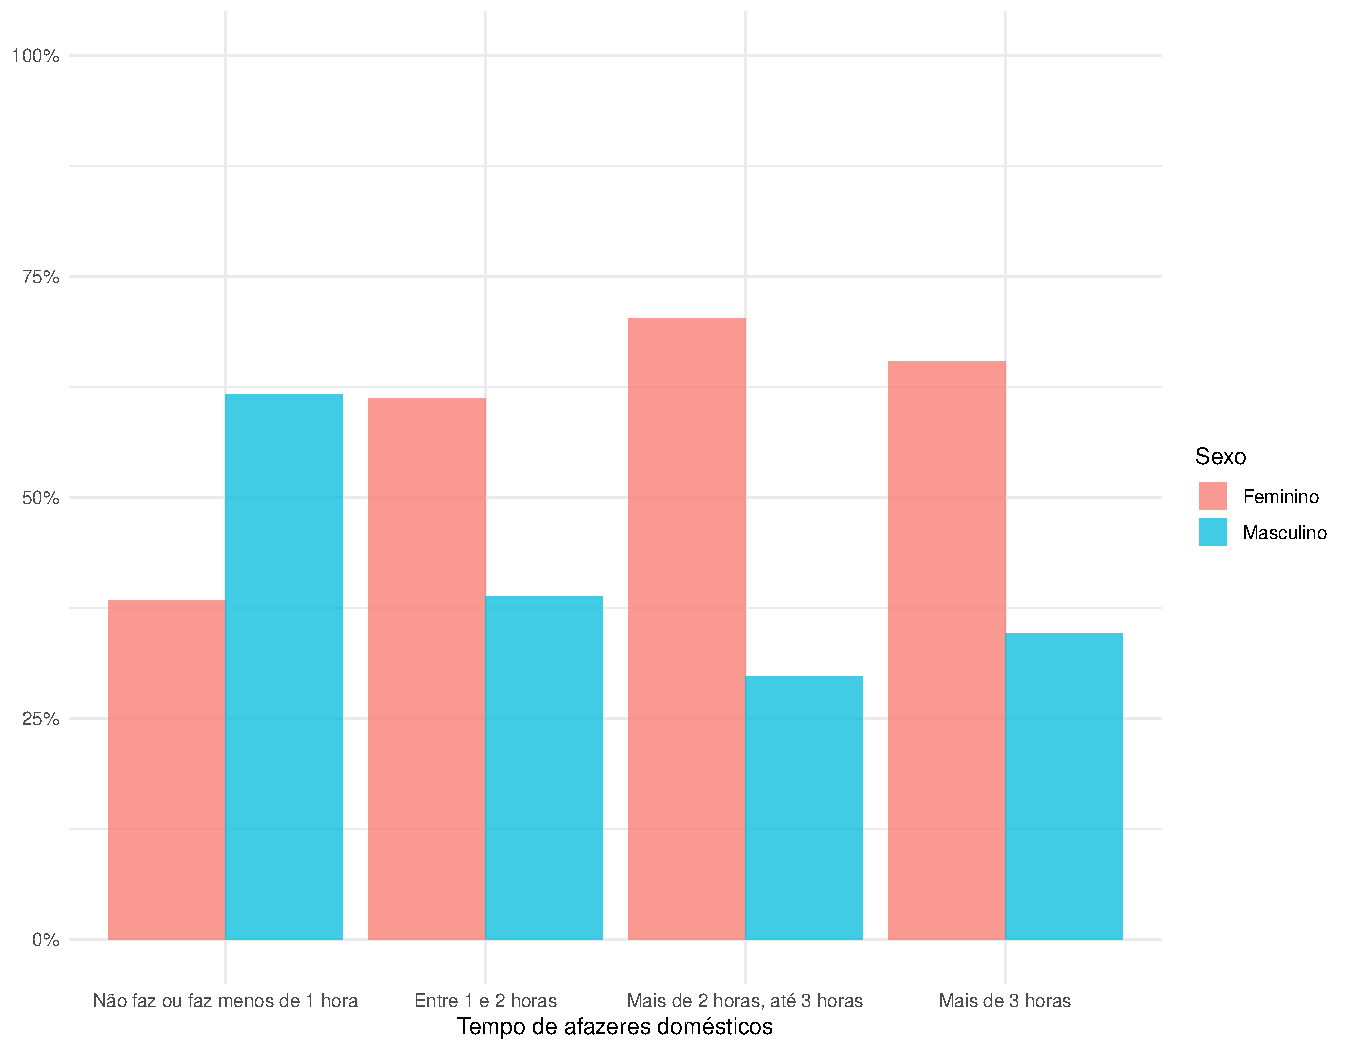
\includegraphics[width=16cm]{img/sexo_afazeres.pdf}
    \end{center}
    \fonte{Amostra de 5.271 alunos do 9\textsuperscript{o} ano do SAEB 2017.}
    \nota{Amostra retirada de uma amostragem aleatórias simples.}
\end{figure}

A \autoref{sexo_afazeres} apresenta como se distribuem estes períodos em relação ao sexo
do aluno, no qual estudantes do sexo feminino tendem a gastar mais tempo com atividades
domésticas. O único período em que o sexo feminino teve
menos representatividade foi a  categoria que menos tempo diário é gasto com atividades domésticas,
“Não faz ou faz menos de 1 hora”.

Para os períodos em que pelo menos uma hora por dia é gasta, o sexo feminino
representa no mínimo 60\% de todos os indivíduos, o que pode indicar que a proporção 
de estudantes do sexo masculino possui mais disponibilidade de tempo em casa para estudos.

%%%%% Gráfico de Escolaridade da mãe por afazeres_domesticos
\begin{figure}[h]
    \caption{Proporção total do nível de escolaridade da mãe
    com base nos períodos de tempo de afazeres domésticos por parte dos alunos.\label{esc_mae_afazeres}}
    \begin{center}
        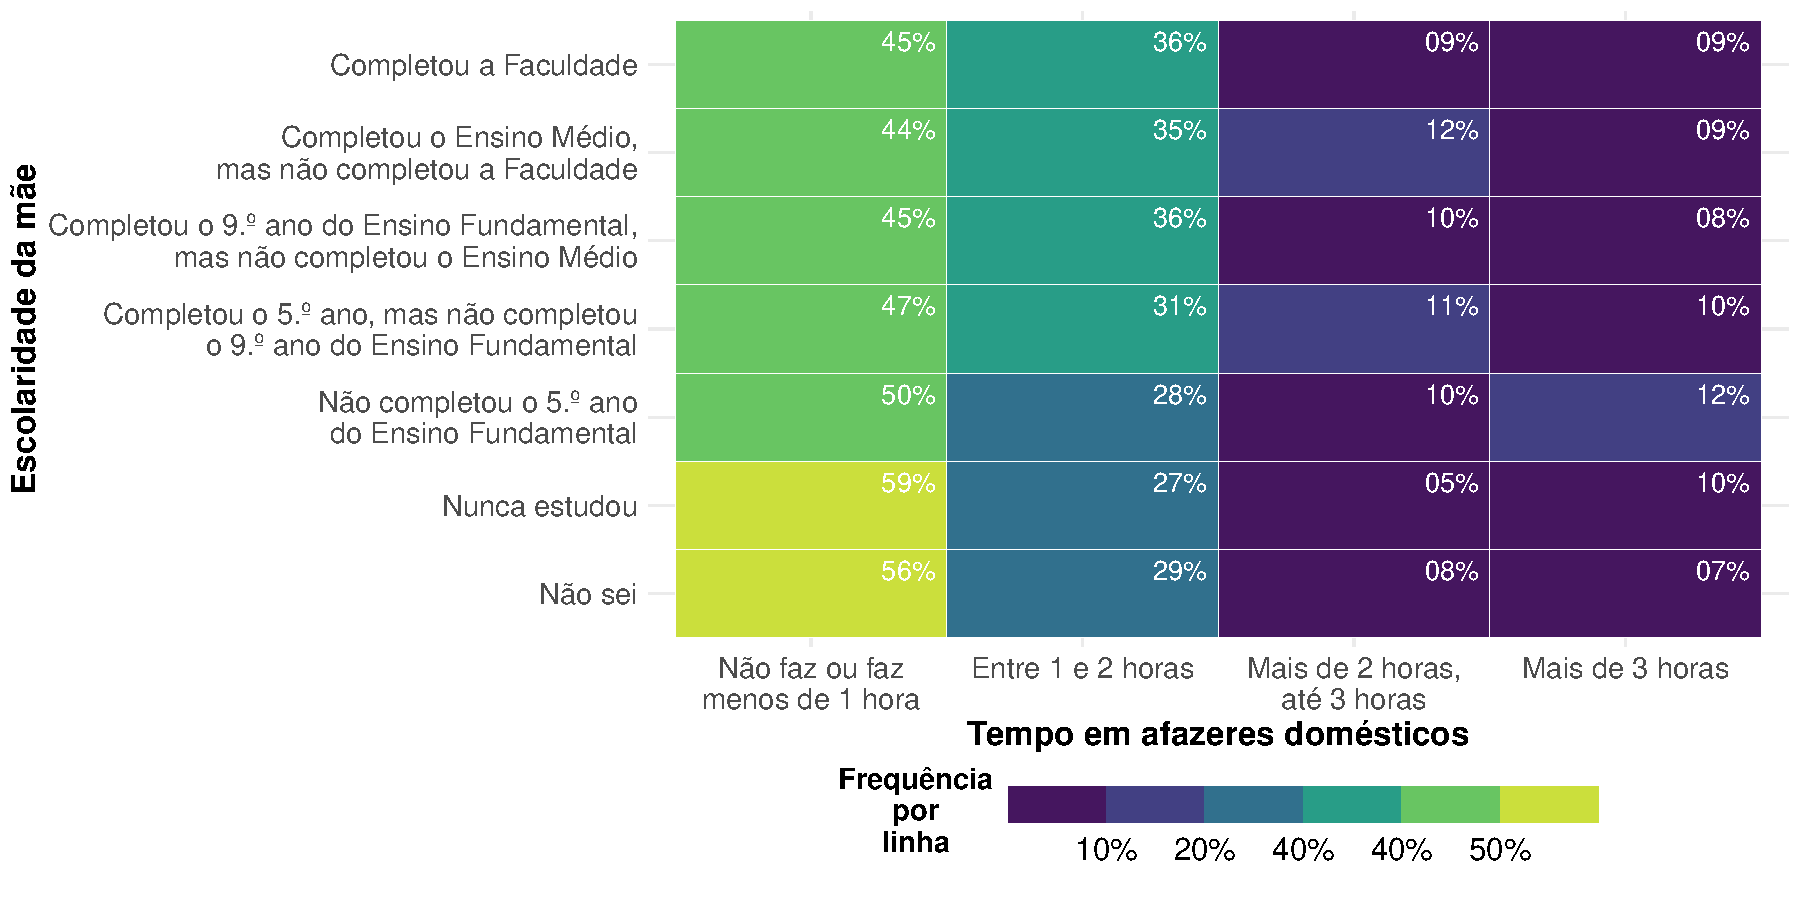
\includegraphics[width=16cm]{img/esc_mae_afazeres.pdf}
    \end{center}
    \fonte{Amostra de 5.271 alunos do 9\textsuperscript{o} ano do SAEB 2017.}
    \nota{Amostra retirada de uma amostragem aleatórias simples.}
\end{figure}

Outras observações sobre tempo gasto podem ser feitas ao observar a \autoref{esc_mae_afazeres},
que mostra o tempo gasto pelos alunos com atividades domésticas pra cada nível de escolaridade da mãe.
Ao analisar, a proporção de alunos que exercem estas atividade, sobre o total de alunos para cada nível
desta escolaridade, apresenta pelo menos 70\% localizado entre o período de tempo que 
não fazem ou fazem até 2 horas.
%%%%%%%%%%%%%%%%%%%%%%% Tabelas %%%%%%%%%%%%%%%%%%%%%%%%%%%%%%%%%%%%%%%%%%%%%%%%%%%%%%%%%%%%%%%%%

Nos testes estatísticos, que avaliam a hipótese de igualdade das distribuições, com base nesses afazeres (\autoref{tab:af_test}) e com a
confiança de 95\%, a variável sexo obteve evidências significativas para afirmar que o tempo
médio não é igual entre os sexos, no qual o sexo feminino possui
proporções superiores em períodos de tempo maiores nestas atividades.

Ao testar a variável raça/cor dos alunos sob a mesma hipótese, não foram obtidas evidências significativas,
apontando que não há indícios de diferenças, em média, entre as raças/cores, no tempo gasto
nestes afazeres, assim como para a variável sobre a escolaridade da mãe com estes afazeres.



%%%%% Tabela dos testes paras relações com afazeres domesticos

\begin{table}[htb]
    \caption{Testes de igualdade na variabilidade sobre as relações 
            com o tempo de afazeres domésticos por parte dos alunos.\label{tab:af_test}}
        \centering
        \begin{tabular}{cccc}
        \toprule
        Teste & $H_0$& P-valor & Decisão de $H_0$ (95\%)\\
        \midrule \midrule
        K & $\mu_{Raça/Cor}$ iguais & 0.369 & Aceita\\
        K & $\mu_{Esc(mãe)}$ iguais & Aprox. 0 & Rejeita\\
        W & $\mu_M = \mu_F$ iguais & Aprox. 0 & Rejeita\\
        \bottomrule
        \end{tabular}
        \fonte{Amostra de 5.271 alunos do 9\textsuperscript{o} ano do SAEB 2017.}
        \nota{Amostra retirada de uma amostragem aleatória simples.}
        \nota[Anotações]{Os subíndices M e F referem-se, respectivamente, aos sexos Masculino e Feminino
        dos alunos. Esc (mãe) diz respeito à escolaridade da mãe destes. O Aprox. 0 refere-se a um número
        muito pequeno considerado por este estudo aproximadamente zero.}
\end{table}



%%%%% Tabela de comparação da escolaridade da mãe com afazeres domesticos
O teste realizado com base na escolaridade da mãe sobre o tempo em afazeres domésticos, obteve evidências significativas sobre a
existência de diferença no tempo gasto com afazeres domésticos. Ao efetuar testes pareados para cada 
nível escolar da mãe com a confiança de 95\% (\autoref{tab:esc_mae_afzr}) sobre essa mesma hipótese de igualdade, a proporção de alunos que gastam tempo nestes
afazeres, obteve diferenças nas distribuições apenas para aqueles que responderam não saber a escolaridade mãe com
os outros níveis desta escolaridade, exceto para aqueles que a mãe nunca estudou obteve igualdade.  
\clearpage

\begin{table}[htb]
    \centering
\caption{Comparações dois a dois entre as ordens das posições sobre os tempos de afazeres domésticos
com base na escolaridade das mães dos alunos\label{tab:esc_mae_afzr}}
    \begin{tabular}{lcc}
    \toprule
    Comparações & P-valor & Evidência (RA 95\%)\\
    \midrule \midrule
    Não sabe = Nunca estudou & 1.0000 & Iguais\\
    Não sabe = Incompleto 5.\textsuperscript{o} ano do EF  & 0.0078 & Desiguais\\
    Não sabe = Completou 5.\textsuperscript{o} ano do EF  & 0.0005 & Desiguais\\
    Não sabe = Completou 9.\textsuperscript{o} ano do EF  & 0.0001 & Desiguais\\
    Não sabe = Completou EM & Aprox. 0 & Desiguais\\
    Não sabe = Completou Faculdade & 0.0011 & Desiguais\\
    
    Nunca estudou = Incompleto 5.\textsuperscript{o} ano do EF  & 1.0000 & Iguais\\
    Nunca estudou = Completou 5.\textsuperscript{o} ano do EF  & 0.5598 & Iguais\\
    Nunca estudou = Completou 9.\textsuperscript{o} ano do EF  & 0.4165 & Iguais\\
    Nunca estudou = Completou EM & 0.1114 & Iguais\\
    Nunca estudou = Completou Faculdade & 0.4707 & Iguais\\
    
    Incompleto 5.\textsuperscript{o} ano do EF = Completou 5.\textsuperscript{o} ano do EF  & 1.0000 & Iguais\\
    Incompleto 5.\textsuperscript{o} ano do EF = Completou 9.\textsuperscript{o} ano do EF  & 1.0000 & Iguais\\
    Incompleto 5.\textsuperscript{o} ano do EF = Completou EM & 1.0000 & Iguais\\
    Incompleto 5.\textsuperscript{o} ano do EF = Completou Faculdade & 1.0000 & Iguais\\
    
    Completo 5.\textsuperscript{o} ano do EF = Completou 9.\textsuperscript{o} ano do EF  & 1.0000 & Iguais\\
    Completo 5.\textsuperscript{o} ano do EF = Completou EM & 1.0000 & Iguais\\
    Completo 5.\textsuperscript{o} ano do EF = Completou Faculdade & 1.0000 & Iguais\\
    
    Completo 9.\textsuperscript{o} ano do EF = Completou EM & 1.0000 & Iguais\\
    Completo 9.\textsuperscript{o} ano do EF = Completou Faculdade & 1.0000 & Iguais\\
    
    Completou EM = Completou Faculdade & 1.0000 & Iguais\\
    \bottomrule
    \end{tabular}
    \centering
    \fonte{Amostra de 5.271 alunos do 9\textsuperscript{o} ano do SAEB 2017.}
    \nota{Amostra retirada de uma amostragem aleatória simples. Teste de Wilcoxon dois a dois efetuado com a correção de 
    Bonferroni no P-valor.}
    \nota[Anotações]{Aprox. 0 refere-se à algum número muito pequeno considerando aproximadamente zero.
                    O EF e EM remete ao ensino fundamental e ensino médio respectivamente.}
\end{table}

\newpage
%%%%%%%%%%%%%%%%%%%%%%%%%%%%%%%%%%%%%%%%%%%%%%%%%%%%%%%%%%%%%%%%%%%%%%%%%%%%%%%%%%%%%%%%%%%%%%%%%%%%%%%%%%%
%%%%%%%%%%%%%%%%%%%%%%%%%%%%%%%%% NOTAS %%%%%%%%%%%%%%%%%%%%%%%%%%%%%%%%%%%%%%%%%%%%%%%%%%%%%%%%%%%%%%%%%%%%%%%%%
%%%%%%%%%%%%%%%%%%%%%%%%%%%%%%%%%%%%%%%%%%%%%%%%%%%%%%%%%%%%%%%%%%%%%%%%%%%%%%%%%%%%%%%%%%%%%%%%%%%%%%%%%%%
\section{Notas}

Para medir o desempenho dos alunos no aprendizado básico, a soma das notas em Língua Portuguesa e Matemática da
Prova Brasil foi utilizado para verificar se há indícios de desigualdade com algum grupo das
relações abordadas pelo estudo.

%%%%%%%%%%%%%%%%%%%%%%% Graficos %%%%%%%%%%%%%%%%%%%%%%%%%%%%%%%%%%%%%%%%%%%%%%%%%%%%%%%%%%%%%%%%%
%%%%% Grafico com raca cor e notas
\begin{figure}[h]
    \caption{Distribuições das somas das notas com base na raça/cor dos alunos.\label{fig:raca_cor_notas}}
    \begin{center}
        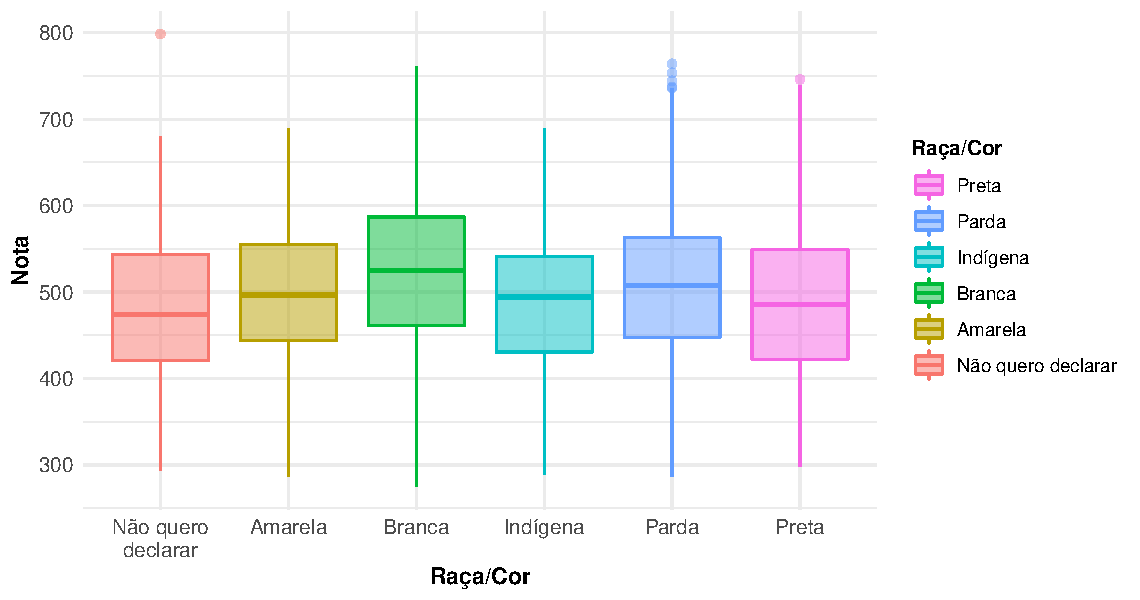
\includegraphics[width=16cm]{img/raca_cor_notas.pdf}
    \end{center}
    \fonte{Amostra de 5.271 alunos do 9\textsuperscript{o} ano do SAEB 2017.}
    \nota{Amostra retirada de uma amostragem aleatórias simples.}
\end{figure}
Sobre a \autoref{fig:raca_cor_notas}, nota-se que a soma das notas dos grupos tem uma
tendência da medida central (50\% dos alunos) ser localizada na nota 500, que varia pouco de 
acordo com a raça, sendo o fenótipo Branco aquele que possui as maiores valores nas medidas
de posição sobre as estas notas.

A raça Parda é a que possui o maior número de outliers entre os estudantes,
mas a maior nota observada esteve presente no grupo que não quis declarar a raça/cor.

\newpage
%%%% Grafico localizacao com notas

\begin{figure}[htb]
    \caption{Distribuições empíricas das somas das notas com base nas localizações das
    das escolas dos alunos.\label{img:loc_notas}}
    \begin{center}
        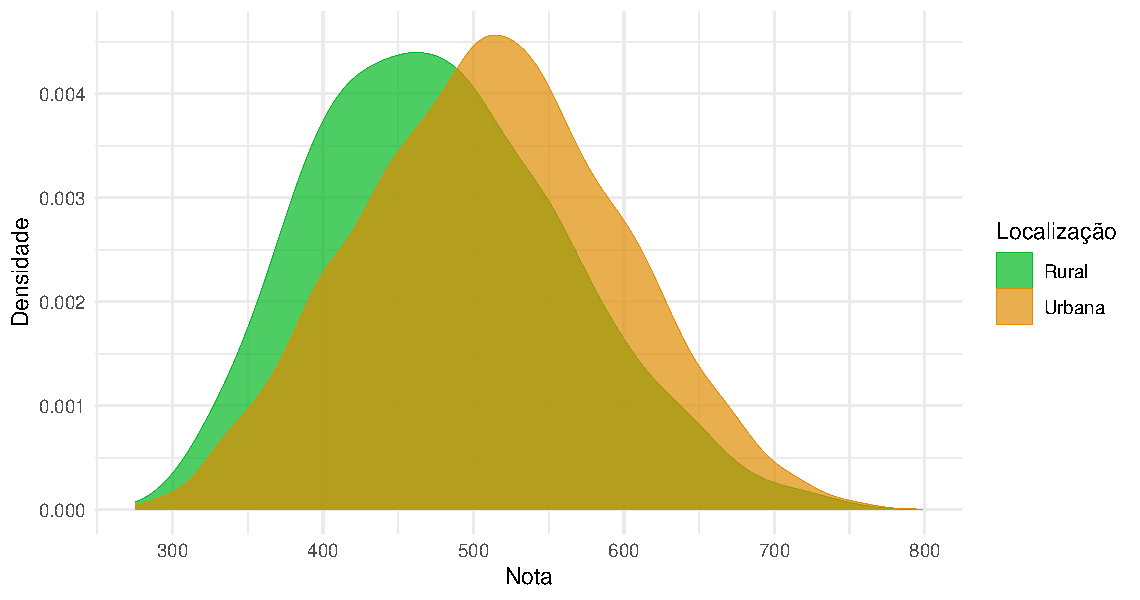
\includegraphics[width=16cm]{img/loc_notas.pdf}
    \end{center}
    \fonte{Amostra de 5.271 alunos do 9\textsuperscript{o} ano do SAEB 2017.}
    \nota{Amostra retirada de uma amostragem aleatórias simples.}
\end{figure}

Na \autoref{img:loc_notas}, é possível observar um grau de assimetria um pouco maior nestas notas para as escolas
das regiões rurais em relação às regiões urbanas. A distribuição das notas nas regiões rurais foi um pouco mais inclinada
para a esquerda e com moda inferior à moda das zonas urbanas, que possui uma distribuição mais centralizada.

As escolas rurais apresentaram uma nota média de 479, que também é inferior quando comparada com a nota média das
escolas urbanas, que foi de 512.

%%%%% Grafico da escolaridade da mae com notas

Para a \autoref{img:esc_mae_notas}, observa-se um crescimento das notas em geral, à medida que o grau de escolaridade
das mães é maior, de modo que apenas aqueles alunos que responderam que desconhecem a escolaridade da mãe
tiveram comportamento independente a essa observação. Esse comportamento é observado de forma equivalente aos valores extremos,
onde a maior nota registrada vem por parte do aluno cuja mãe completou a faculdade.
\newpage

\begin{figure}[h]
    \caption{Distribuições das somas das notas com base nas escolaridades 
    das mães dos alunos\label{img:esc_mae_notas}}
    \begin{center}
        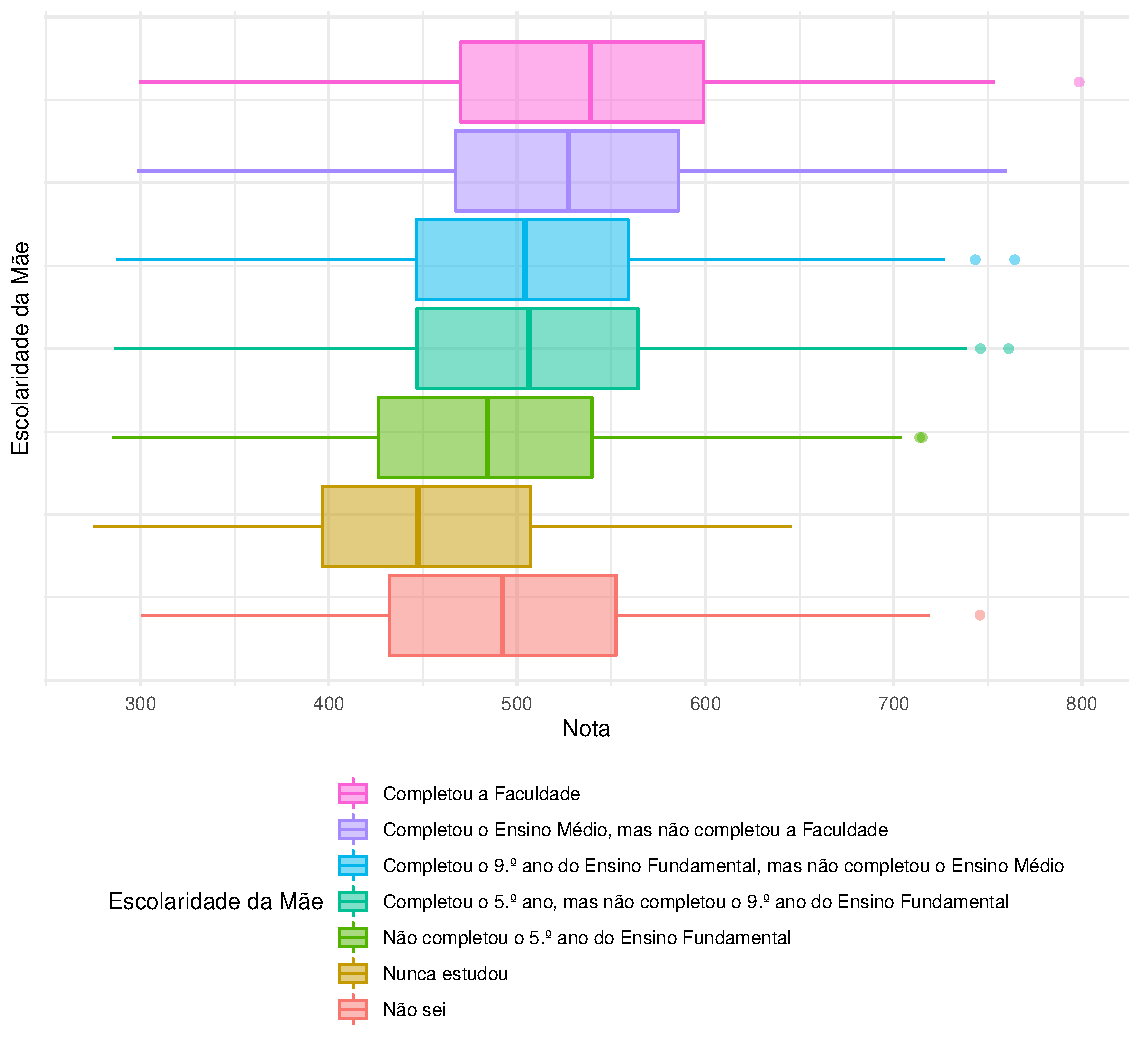
\includegraphics[width=16cm]{img/esc_mae_notas.pdf}
    \end{center}
    \fonte{Amostra de 5.271 alunos do 9\textsuperscript{o} ano do SAEB 2017.}
    \nota{Amostra retirada de uma amostragem aleatórias simples.}
\end{figure}





%%%%%%%%%%%%%%%%%%%%%%% Tabelas %%%%%%%%%%%%%%%%%%%%%%%%%%%%%%%%%%%%%%%%%%%%%%%%%%%%%%%%%%%%%%%%%
Ao realizar testes sobre a soma das notas, foi verificado se havia indícios de diferenças significativas entre as médias
da soma das notas com base nas relação efetuada pelo estudo, com a confiança 95\%.
Para efetuar estes testes, foi avaliado primeiramente a hipótese de igualdade sobre as variâncias
das notas (Teste B) para cada relação abordada pelo estudo como as localizações das escolas, 
escolaridade da mãe, sexo e a raça/cor do aluno, no qual apenas a relação com o sexo rejeita esta hipótese
como demostrado na \autoref{tab::tests_notas}.

\newpage
%%%%%% Tabela com testes para as relacoes das notas
\begin{table}[htb]
\caption{Testes para as relações com soma
 das notas dos alunos.\label{tab::tests_notas}}
    \centering
    \begin{tabular}{cccc}
    \toprule
    Teste & $H_0$& P-valor & Decisão de $H_0$ (95\%)\\
    \midrule \midrule
    B & $\sigma_R^2 = \sigma_U^2$ & 0.503 & Aceita\\
    B & $\sigma_M^2 = \sigma_F^2$ & 0.002 & Rejeita\\
    B & $\sigma_{Raça/Cor}^2$ iguais & 0.265 & Aceita\\
    B & $\sigma_{Esc(mãe)}^2$ iguais & 0.132 & Aceita\\
    T & $\mu_R = \mu_U$ & Aprox. 0 & Rejeita\\
    T & $\mu_M = \mu_F$ & 0.905 & Aceita\\
    ANOVA & $\mu_{Raça/Cor}$ iguais & Aprox. 0 & Rejeita\\
    ANOVA & $\mu_{Esc(mãe)}$ iguais & Aprox. 0 & Rejeita\\
    \bottomrule
    \end{tabular}
    \fonte{Amostra de 5.271 alunos do 9\textsuperscript{o} ano do SAEB 2017.}
    \nota{Amostra retirada de uma amostragem aleatória simples. Teste T dois a dois efetuado com a correção de 
    Bonferroni no P-valor.}
    \nota[Anotações]{Os subíndices, com base nos alunos, $R$ e $U$ referem-se às localizações
                    das escolas rurais e urbanas, M e F sobre os sexos Masculino e Feminino
                    respectivamente e Esc(mãe) diz respeito à escolaridade da mãe. 
                    O Aprox. 0 refere-se à algum número 
                    muito pequeno considerado por este estudo aproximadamente zero.}
\end{table}

% analise dos testes (tabela tab::tests_notas)
Ao concluir sobre estas relações com as variâncias na \autoref{tab::tests_notas}, foram avaliadas as
hipóteses de igualdades destas médias, que pelo mesmo nível de confiança. Houveram indícios de igualdade 
com base nos sexos (Teste T), que diz sobre não existir diferença em média entre as notas dos sexos masculino e feminino.

Sobre a hipótese de igualdade de notas por raça/cor do aluno, e a escolaridade da mãe (Teste ANOVA)
sobre essas notas, houveram indícios significativos de diferença nas médias em alguma destas relações,
onde os testes dois a dois (Teste T) são apropriados para investigar que diferenças foram essas.

Para a relação com as localizações das escolas, a hipótese de igualdade também foi rejeitada, e as escolas 
urbanas obteiveram, em média, um valor superior às escolas rurais.


\newpage
%%%%%% Tabela de comparacao entre raca/cor e notas

\begin{table}[htb]
    \centering
\caption{Comparações dois a dois entre as médias sobre a soma das notas
        com base na raça/cor dos alunos.\label{tab:raca_cor_notas}}
    \begin{tabular}{lcc}
    \toprule
    Comparações & P-valor & Evidência (RA 95\%)\\
    \midrule \midrule
    Amarela = Não quero declarar & 0.4113 & Iguais\\
    Amarela = Branca & 0.0005 & Desiguais\\
    Amarela = Indígena & 1.0000 & Iguais\\
    Amarela = Parda & 1.0000 & Iguais\\
    Amarela = Preta & 1.0000 & Iguais\\
    Branca = Não quero declarar & Aprox. 0 & Desiguais\\
    Branca = Indígena & 0.0010 & Desiguais\\
    Branca = Parda & Aprox. 0 & Desiguais\\
    Branca = Preta & Aprox. 0 & Desiguais\\
    Indígena = Não quero declarar & 1.0000 & Iguais\\
    Indígena = Parda & 0.7758 & Iguais\\
    Indígena = Preta & 1.0000  & Iguais\\
    Parda = Não quero declarar & Aprox. 0 & Desiguais\\
    Parda = Preta & Aprox. 0 & Desiguais\\
    \bottomrule
    \end{tabular}
    \centering
    \fonte{Amostra de 5.271 alunos do 9\textsuperscript{o} ano do SAEB 2017.}
    \nota{Amostra retirada de uma amostragem aleatória simples. Teste T dois a dois efetuado com a correção de 
    Bonferroni no P-valor.}
    \nota[Anotações]{Aprox. 0 refere-se à algum número muito pequeno considerando aproximadamente zero.}
    
\end{table}

Na \autoref{tab:raca_cor_notas}, as comparações dois a dois apresentaram que a raça/cor branca obteve diferença,
nestes testes de hipótese de igualdade das médias, entre todas as outras raças, confirmando o que a 
\autoref{fig:raca_cor_notas} apontava.

As únicas desigualdades dessa hipótese que não foram entre as comparações com os indivíduos da raça/cor branca
foram entre os alunos pardos com os pretos e aqueles que não quiseram declarar.

Todos os outros testes não só levam à aceitação da hipótese de igualdade das médias ($H_0$), como apresentaram um p-valor
significativamente alto, que diz respeito a níveis de confiabilidade elevados.


%%%%% Tabela de comparação da notas com Escolaridade da mae
As hipóteses iniciais para a variável do nível de escolaridade da mãe são passadas como comparações dois a dois na \autoref{tab:esc_mae_notas},
que supõe esta hipóteses de igualdade entre as médias da soma das nota dos alunos, com cada grupo de nível escolar das mães.
\newpage

\begin{table}[htb]
    \centering
\caption{\label{tab:esc_mae_notas}Comparações dois a dois das notas entre os alunos com base na escolaridade da mãe}
    \begin{tabular}{lcc}
    \toprule
    Comparações & P-valor & Evidência (RA 95\%)\\
    \midrule \midrule
    Não sabe = Nunca estudou & Aprox. 0 & Desiguais\\
    Não sabe = Incompleto 5.\textsuperscript{o} ano do EF  & 1.0000 & Iguais\\
    Não sabe = Completou 5.\textsuperscript{o} ano do EF  & 0.0084 & Desiguais\\
    Não sabe = Completou 9.\textsuperscript{o} ano do EF  & 0.1927 & Iguais\\
    Não sabe = Completou EM & Aprox. 0 & Desiguais\\
    Não sabe = Completou Faculdade & Aprox. 0 & Desiguais\\
    Nunca estudou = Incompleto 5.\textsuperscript{o} ano do EF  & 0.0038 & Desiguais\\
    Nunca estudou = Completou 5.\textsuperscript{o} ano do EF  & Aprox. 0 & Desiguais\\
    Nunca estudou = Completou 9.\textsuperscript{o} ano do EF  & Aprox. 0 & Desiguais\\
    Nunca estudou = Completou EM & Aprox. 0 & Desiguais\\
    Nunca estudou = Completou Faculdade & Aprox. 0 & Desiguais\\
    Incompleto 5.\textsuperscript{o} ano do EF = Completou 5.\textsuperscript{o} ano do EF  & 0.0002 & Desiguais\\
    Incompleto 5.\textsuperscript{o} ano do EF = Completou 9.\textsuperscript{o} ano do EF  & 0.0048 & Desiguais\\
    Incompleto 5.\textsuperscript{o} ano do EF = Completou EM & Aprox. 0 & Desiguais\\
    Incompleto 5.\textsuperscript{o} ano do EF = Completou Faculdade & Aprox. 0 & Desiguais\\
    Completo 5.\textsuperscript{o} ano do EF = Completou 9.\textsuperscript{o} ano do EF  & 1.0000 & Iguais\\
    Completo 5.\textsuperscript{o} ano do EF = Completou EM & Aprox. 0 & Desiguais\\
    Completo 5.\textsuperscript{o} ano do EF = Completou Faculdade & Aprox. 0 & Desiguais\\
    Completo 9.\textsuperscript{o} ano do EF = Completou EM & Aprox. 0 & Desiguais\\
    Completo 9.\textsuperscript{o} ano do EF = Completou Faculdade & Aprox. 0 & Desiguais\\
    Completou EM = Completou Faculdade & 1.0000 & Iguais\\
    \bottomrule
    \end{tabular}
    \centering
    \fonte{Amostra de 5.271 alunos do 9\textsuperscript{o} ano do SAEB 2017.}
    \nota{Amostra retirada de uma amostragem aleatória simples. Teste T dois a dois efetuado com a correção de 
    Bonferroni no P-valor.}
    \nota[Anotações]{Aprox. 0 refere-se à algum número muito pequeno considerando aproximadamente zero e 
    EF e EM remete ao ensino fundamental e ensino médio respectivamente.}
    
  \end{table}

E dentre esses grupos, somente os grupos que aqueles alunos que declararam não saber a escolaridade da mãe com aquelas mães que tem o
5\textsuperscript{o} incompleto ou 9\textsuperscript{o} completo, aquelas mães que tem completo o 5\textsuperscript{o} com as que tem
9\textsuperscript{o}, com base no ensino fundamental, e aquelas que tem completo o ensino médio com as que as que possui a 
faculdade completa, esta hipótese foi rejeitada, com um nível de significância de 95\%. Ao considerar estas igualdades e 
as outras desigualdades das médias sobre a soma destas notas, há maiores valores para aquelas mães que possuem
níveis de escolaridade superiores.
  
  % ---
  % == PARTE - Finaliza a parte no bookmark do PDF
  %    para que se inicie o bookmark na raiz e adiciona espaço de parte no Sumário
  \phantompart
  
  % ---
  % Conclusão
  %----------------------------------------------------------------------------------------------------------------
% File : conclusao.tex
%----------------------------------------------------------------------------------------------------------------

% ---
% Conclusão
\chapter{Conclusão}


\begin{itemize}

\item A variável Raça/Cor não exerce influência no tempo de afazeres domésticos.
\item A variável Escolaridade da Mãe exerce influência no tempo de afazeres domésticos.
\item A variável Sexo exerce influência no tempo de afazeres domésticos.
\item A proporção de alunos que gastam tempo com afazeres domésticos, cujo as mães que nunca estudaram se difere com todos os outros níveis escolares que, em grande parte gastam menos de uma hora.
\item O mesmo se observa para as mães com o 5º ano incompleto, no qual o único grau que não se difere é dos alunos que responderam que não sabiam sobre o nível educacional da mãe.
\item Não existe diferença sobre as médias das notas dos estudantes de acordo com o sexo.
\item A média das notas dos estudantes varia de acordo com a Raça/Cor e com o nível de escolaridade da mãe.
\item Há uma clara desigualdade entre as notas por raça quando se compara a branca com as demais, e quase todas as desigualdades derivaram dela.
\item As únicas desigualdades que não foram entre comparações de indivíduos de cor branca com outros foi a comparação entre indivíduos pardos e pretos, e também acomparação entre indivíduos pardos e aqueles que não quiseram declarar.
\item Somente aqueles que declararam não saber a escolaridade da mãe tiveram suas hipóteses de igualdade das médias rejeitadas, indicando diferença entre as notas médias desses estudantes com aqueles cujas mães completaram o EnsinoFundamental I e II, ensino médio e faculdade. A única hipótese de igualdade das notas desses estudantes aceita foi a com estudantes cujas mães nunca haviam estudado.


\end{itemize}
  
  % ----------------------------------------------------------
  % == ELEMENTOS PÓS-TEXTUAIS
  % ----------------------------------------------------------
  \postextual
  
  % ----------------------------------------------------------
  % Referências bibliográficas
  \bibliography{bib/referencia}
  
  % ----------------------------------------------------------
  % Glossário
  % Consulte o manual da classe abntex2 para orientações sobre o glossário.
  %\glossary
  
  % ----------------------------------------------------------
  % == APÊNDICES
  % ----------------------------------------------------------

  % ---
  % Inicia os apêndices
 
  
  % ----------------------------------------------------------
  % == ANEXOS
  % ----------------------------------------------------------
  
  % ---
  % Inicia os anexos
  % ---
  \begin{anexosenv}
    
    % Imprime uma página indicando o início dos anexos
    \partanexos
    % ---
    % Anexos (incluir os arquivos com os anexos)
    %----------------------------------------------------------------------------------------------------------------
% File : anexo1.tex
%----------------------------------------------------------------------------------------------------------------

% Apendice 1
\chapter{Amostra}
Os bancos de dados dos alunos participantes do SAEB de 2017 foram disponibilizados como
amostras de tamanho 2.000 em formato CSV. Cada banco de dados era uma amostra aleatória
diferente do banco de dados original do SAEB, para cada aluno da Turma A
de Métodos Estatísticos 2 do semestre 1/2020 da Universidade de Brasília (UnB).

Os dados utilizados nesse documento foi a junção dos três bancos de dados dos integrantes com
a retirada dos alunos que detinham a $NA's$, nestas amostras com os seguintes nomes: \textbf{amostra\_190015853.csv}, \textbf{amostra\_190029498.csv} e 
\textbf{amostra\_190127180.csv}
  
  \end{anexosenv}
  
  %---------------------------------------------------------------------
  % == INDICE REMISSIVO
  %---------------------------------------------------------------------
  \phantompart
  
  
  %---------------------------------------------------------------------
  % Formulário de Identificação (opcional)
  %---------------------------------------------------------------------
  %\include{postextuais/form_identif}

\end{document}
